%!TEX TS-program = xelatex
\documentclass[a4paper]{adcv}
\usepackage{comment}

\newcommand*{\hib}{}
\newcommand*{\uib}{}
\newcommand*{\uniaq}{}

\addbibresource{musty_cv.bib}

\title{musty_cv}

\adcvname{Michael}{Musty}
\adcvtitle{Ph.D. Candidate, Mathematics, Dartmouth College}
\adcvaddress{55 Church Street}{03779}{Piermont}{New Hampshire USA}
%\adcvwebsite{https://math.dartmouth.edu/~mjmusty}{math.dartmouth.edu/~mjmusty}
\adcvwebsite{https://michaelmusty.github.io}{michaelmusty.github.io}
\adcvemail{michaelmusty}{gmail}{com}
\adcvphone{(+1) 603 728 7903}
\adcvdate{December 2018}
\adcvlinkedin{https://www.linkedin.com/in/mjmusty/}{mjmusty}

\begin{document}

\section{Education}{
  \begin{adcvtabletwo}
    \adcvrowtwo{\textbf{Ph.D. Mathematics}, Dartmouth College, Hanover, New Hampshire, USA}{expected 2019}
    \adcvrowskip
    \adcvrowtwo{\textbf{M.Sc. Mathematics}, University of Vermont, Burlington, Vermont, USA}{2014}
    \adcvrowskip
    \adcvrowtwo{\textbf{B.A. Mathematics/Scientific Computing}, Boston College, Chestnut Hill, Massachusetts, USA}{2008}
  \end{adcvtabletwo}
}

\section{Research Experience}{
  \begin{adcvtabletwo}
    \adcvrowtwo{\textbf{2-Group Belyi Maps}, Ph.D. Thesis}{expected 2019}
    \adcvrowmulti{
      In this thesis, I develop and implement an algorithm to compute a
      database of Galois Belyi maps with monodromy group a 2-group.
      This database contains Belyi maps up to degree 256.
      I use this data to pose conjectures about these objects.
      For instance,
      every 2-group Belyi map up to degree 256 has refined passport size 1,
      and partially proven results point towards the possibility that this
      is true in general.
      In addition to forming conjectures,
      I use this data to search for number fields unramified away from 2.
      \begin{itemize}
        \item
          repository: \url{https://github.com/michaelmusty/solvabledessins}
        \item
          visualization: \url{https://dessin-explorer.org}
      \end{itemize}
    }
    \adcvrowskip
    %\adcvrowtwo{\textbf{Computing TODO Homology}, Programmer}{2019}
    %\adcvrowmulti{
    %}
    %\adcvrowskip
    \adcvrowtwo{\textbf{Computing Canonical Rings of Hilbert Modular Forms}, Programmer}{2018}
    \adcvrowmulti{
      I worked on a large (10 person) team to implement techniques to compute
      canonical rings of Hilbert modular forms.
      I was responsible for the data structure to store and compute with
      Fourier expansions of Hilbert modular forms
      necessary to support these computations.
      \begin{itemize}
        \item
          repository: \url{https://github.com/edgarcosta/hilbertmodularforms}
      \end{itemize}
    }
    \adcvrowskip
    \adcvrowtwo{\textbf{A Database of Belyi Maps}, Co-author}{2018}
    \adcvrowmulti{
      In this paper,
      we compute a database of thousands or Belyi maps up to degree 9.
      On top of the group effort to compute an exhaustive list of Belyi maps,
      my main responsibility in this project was implementing the
      database backend using Magma (see repository below) to save the results.
      I then worked in a team of 4 to migrate the data
      over to the LMFDB (\url{www.lmfdb.org}).
      \begin{itemize}
        \item
          Awarded Selfridge Prize at ANTS-XIII:
          \url{http://www.math.grinnell.edu/~paulhusj/ants2018/index.html}
        \item
          repository: \url{https://github.com/michaelmusty/BelyiDB}
        \item
          LMFDB: \url{http://beta.lmfdb.org/Belyi}
      \end{itemize}
    }
    \adcvrowskip
    \adcvrowtwo{\textbf{Understanding the cost of dermatologic care: A survey study of dermatology providers,
    residents, and patients}, Co-author}{2017}
    \adcvrowmulti{
      Using R, I ran the statistical analysis for survey results in this dermatology study
      and generated Likert scale visualizations to analyze the data.
    }
    \adcvrowskip
    \adcvrowtwo{\textbf{Numerical calculation of three-point branched covers of the projective line},
    Co-author}{2014}
    \adcvrowmulti{
      In this paper, we implement a general numerical method to compute Belyi maps
      using power series expansions of modular forms.
      I implemented code to visualize Belyi maps as
      (equivalent) dessins d'enfants conformally
      embedded in the hyperbolic unit disk.
      %My code produced figures drawn using PSTricks (see Figure \ref{fig:dessin}).
      My code produced figures drawn using PSTricks (see Figure 1).
    }
    \adcvrowskip
    \adcvrowtwo{\textbf{Computing Iwasawa $\lambda$-Invariants},
    M.Sc. Thesis}{2014}
    \adcvrowmulti{
      In my M.Sc. thesis I implemented an algorithm to compute the Iwasawa
      $\lambda$-invariant of an abelian number field in Magma.
      Using these computations, I was able to correct some mistakes in
      the literature.
    }
    \adcvrowskip
    % \adcvrowtwo{\textbf{\href{http://www.arcadia-framework.eu}{ARCADIA}}, a framework for developing highly distributed applications}{2014--2016}
  \end{adcvtabletwo}
}

\section{Publications}{

  \begin{refsection}
    \nocite{ants}
    \nocite{aaron}
    \nocite{belyi}
    \printbibliography[title={Peer-Reviewed Articles}, heading=subbibliography]
  \end{refsection}
  % \href{https://scholar.google.com/citations?user=s1bqnpoAAAAJ}{30+ publications} in peer-reviewed conferences and journals.
}

\section{Selected Talks}{
  \begin{adcvpresentations}
    \adcvpresentation{2-Group Belyi Maps}{\href{https://jointmathematicsmeetings.org/amsmtgs/2217_abstracts/1145-11-2469.pdf}{JMM Special Session on Number Theory, Arithmetic Geometry, and Computation}, Baltimore, MD, January 2019}
    \adcvpresentation{A Database of Belyi Maps}{\href{https://math.mit.edu/~drew/2018Conference/SlidesMusty.pdf}{Simons Collaboration Short Talks}, Cambridge, MA, August 2018}
    \adcvpresentation{2-Group Belyi Maps}{\href{https://archimede.mat.ulaval.ca/MAINE-QUEBEC/mq17.html}{Quebec Maine Number Theory Seminar}, October 2017}
    \adcvpresentation{Computing Iwasawa $\lambda$-Invariants}{\href{https://www.math.dartmouth.edu/~zahlen/}{Dartmouth Number Theory Seminar}, Hanover, NH, February 2015}
  \end{adcvpresentations}
}

\section{Work Experience}{
  \begin{adcvtabletwo}
    \adcvrowtwo{\textbf{Graduate Research and Teaching Assistant},
    Dartmouth College, Hanover, NH, USA}{2014-Present}
    \adcvrowskip
    \adcvrowtwo{\textbf{Graduate Research and Teaching Assistant},
    University of Vermont, Burlington, VT, USA}{2012-2014}
    \adcvrowskip
    \adcvrowtwo{\textbf{Adjunct Professor},
    Norwich University, Northfield, VT, USA}{2011-2013}
    \adcvrowskip
    \adcvrowtwo{\textbf{Seasonal Landscaper},
    JM Landscaping, Bradford, VT, USA}{2000-2011}
    \adcvrowskip
    \adcvrowtwo{\textbf{Shipping Assistant},
    Pleasant View Gardens, Loudon, NH, USA}{2009-2010}
    \adcvrowskip
    \adcvrowtwo{\textbf{Permanent Substitute Teacher},
    Merrimack Valley High School, Penacook, NH, USA}{2009-2010}
    \adcvrowskip
    \adcvrowtwo{\textbf{Graduate Research and Teaching Assistant},
    McGill University, Montreal, QC, Canada}{2008-2009}
    \adcvrowskip
    \adcvrowtwo{\textbf{Misc Laborer},
    Glen Farm, Piermont, NH, USA}{1990-2000}
  \end{adcvtabletwo}
}

\section{Community}{

  \begin{adcvtabletwo}
    \adcvrowtwo{\textbf{Dartmouth Mathematics Youth Summer Program},
    Guest Lecturer, Hanover, NH, USA}{2016}
    \adcvrowmulti{
      I gave four guest lectures on probability and knot theory
      and helped organize this two week summer program.
    }
    \adcvrowskip
    \adcvrowtwo{\textbf{Johns Hopkins Program for Talented Youth},
    Guest Lecturer, Hanover, NH, USA}{2015}
    \adcvrowmulti{
      I gave a guest lecture on group theory.
    }
    \adcvrowskip
    \adcvrowtwo{\textbf{Joshua M. Stimson Math Program},
    Organizer, North Haverhill, NH, USA}{2011-2012}
    \adcvrowmulti{
      I organized a four week long summer program
      for advanced middle school students.
      I was the organizer for the first two years of this summer program.
    }
    \adcvrowskip
  \end{adcvtabletwo}
}

\section{Teaching Experience}

Below is a list of university level courses
(21 classroom courses, 5 online courses)
I have taught at
Dartmouth College,
University of Vermont (UVM),
and
Norwich University,
from 2011 to present.
This list does not include any grading, teaching assistantships,
or summer programs.
\begin{itemize}
  \item
    2018 Fall
    \begin{itemize}
      \item
        (Dartmouth) MATH001 Calculus with Algebra
    \end{itemize}
  \item
    2017 Summer
    \begin{itemize}
      \item
        (Dartmouth) MATH022 Linear Algebra with Applications
        \newline
        \url{https://math.dartmouth.edu/~m22x17/}
    \end{itemize}
  \item
    2016 Fall
    \begin{itemize}
      \item
        (Dartmouth) MATH001 Calculus with Algebra
    \end{itemize}
  \item
    2014 Spring
    \begin{itemize}
      \item (UVM) MATH017B Applications of Finite Mathematics
    \end{itemize}
  \item
    2013 Fall
    \begin{itemize}
      \item (UVM) MATH019K Fundamentals of Calculus I
    \end{itemize}
  \item
    2013 Spring
    \begin{itemize}
      \item (UVM) MATH017B Applications of Finite Mathematics
      \item (Norwich) MA102-G Mathematics: A Liberal Art II
      \item (Norwich) MA232-L Elementary Statistics (online)
    \end{itemize}
  \item
    2012 Fall
    \begin{itemize}
      \item (UVM) MATH019H Fundamentals of Calculus I
      \item (Norwich) MA101-B Mathematics: A Liberal Art I
      \item (Norwich) MA212-A Finite Mathematics
      \item (Norwich) MA212-B Finite Mathematics
      \item (Norwich) MA232-L Elementary Statistics (online)
    \end{itemize}
  \item
    2012 Summer
    \begin{itemize}
      \item (Norwich) MA102-A Mathematics: A Liberal Art II (online)
      \item (Norwich) MA232-L Elementary Statistics (online)
    \end{itemize}
  \item
    2012 Spring
    \begin{itemize}
      \item (Norwich) MA107-C Precalculus Mathematics
      \item (Norwich) MA232-A Elementary Statistics
      \item (Norwich) MA232-E Elementary Statistics
      \item (Norwich) MA232-G Elementary Statistics
    \end{itemize}
  \item
    2011 Fall
    \begin{itemize}
      \item (Norwich) MA101-A Mathematics: A Liberal Art I
      \item (Norwich) MA101-E Mathematics: A Liberal Art I
      \item (Norwich) MA107-B Precalculus Mathematics
      \item (Norwich) MA232-L Elementary Statistics (online)
    \end{itemize}
  \item
    2011 Spring
    \begin{itemize}
      \item (Norwich) MA102-G Mathematics: A Liberal Art II
      \item (Norwich) MA102-K Mathematics: A Liberal Art II
      \item (Norwich) MA108-B Applied Calculus
    \end{itemize}
\end{itemize}

\begin{figure}[ht]\label{fig:dessin}
  \centering
  %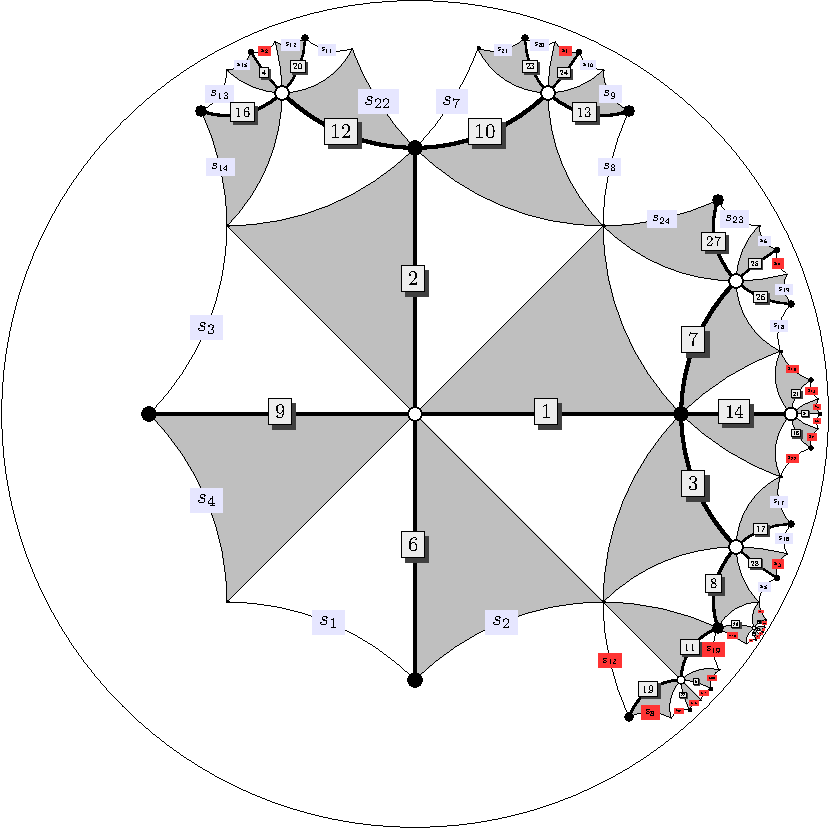
\includegraphics[scale=0.67]{32S2-g5.pdf}
  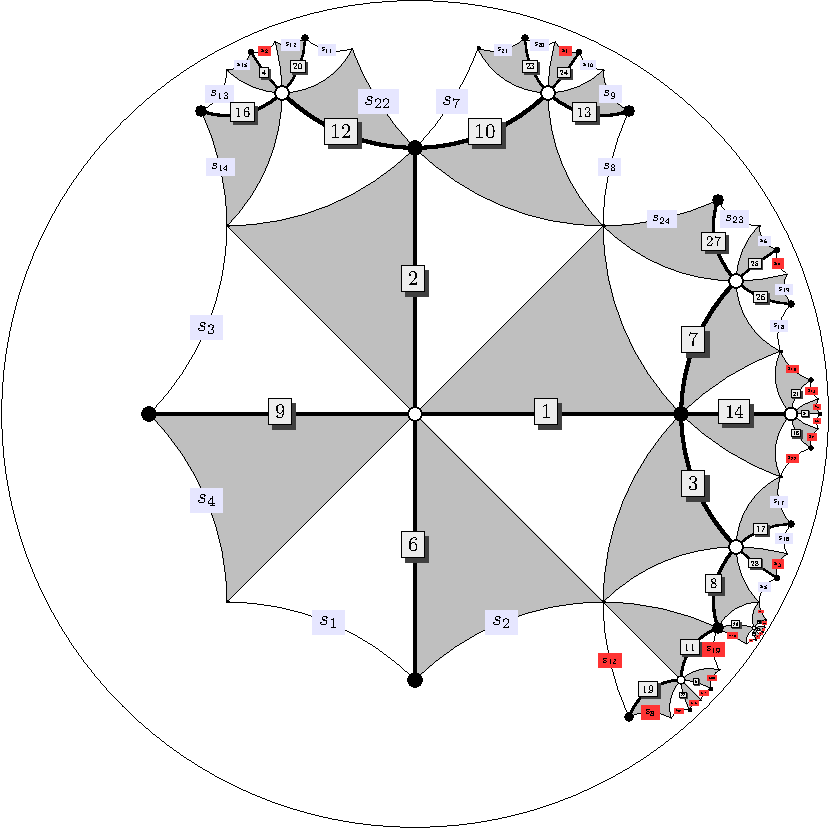
\includegraphics[scale=0.4]{32S2-g5.pdf}
  \caption{
    A genus 5 dessin d'enfant drawn using \LaTeX and PSTricks.
  }
\end{figure}

\end{document}
